% \section{Platform-Server API}
\section{Platform-Server API}

% Its index.ts is:

index.ts 如下:

\begin{minted}{typescript}
// This file is not used to build this module. It is only used during editing
// by the TypeScript language service and during build for verification.
// `ngc` replaces this file with production index.ts when it rewrites private
// symbol names.

export * from './public_api';
\end{minted}


% Its public\_api.ts file is:

它的 public\_api.ts 文件如下:

\begin{minted}{typescript}
/**export {
 * @module
 * @description
 * Entry point for all public APIs of this package.
 */
export * from './src/platform-server';
// This file only reexports content of the `src` folder. Keep it that way.
\end{minted}


% Its src/platfrom-server.ts file (that’s a hyphen rather than an underscore) is:

它的 src/platfrom-server.ts 文件(这是一个连字符而不是下划线)如下:

\begin{minted}{typescript}
export { PlatformState } from './platform_state';
export { ServerModule, platformDynamicServer, platformServer } from './server';
export {
  BEFORE_APP_SERIALIZED,
  INITIAL_CONFIG,
  PlatformConfig,
} from './tokens';
export { ServerTransferStateModule } from './transfer_state';
export { renderModule, renderModuleFactory } from './utils';
export * from './private_export';
export { VERSION } from './version';
\end{minted}


% The main src directory for Platform-Server also contains this private\_export.ts file:

Platform-Server 主要的 src 目录也包含这个 private\_export.ts 文件:

\begin{minted}{typescript}
export {
  INTERNAL_SERVER_PLATFORM_PROVIDERS as ɵINTERNAL_SERVER_PLATFORM_PROVIDERS,
  SERVER_RENDER_PROVIDERS as ɵSERVER_RENDER_PROVIDERS,
} from './server';
export { ServerRendererFactory2 as ɵServerRendererFactory2 } from './server_renderer';
\end{minted}


% The exported API of the Platform-Server package can be represented as:

Platform-Server 包的导出 API 表示\fref{fig:platform_server_public_api}:

\begin{figure}[!hbt]
  \centering
  \caption{Platform-Server Public API}
  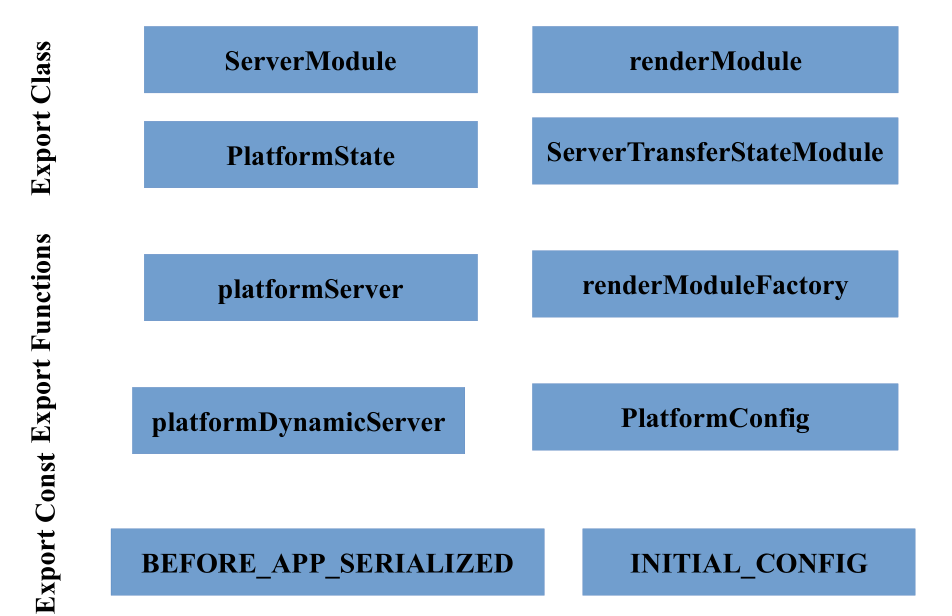
\includegraphics[width=0.75\linewidth]{10_the_platform_server_package/platform_server_public_api}
  \label{fig:platform_server_public_api}
\end{figure}

% \texttt{ServerModule}
% represents the
% \texttt{NgModule}
% for this module.
% \texttt{platformServer()}
% uses the
% offline compiler.
% \texttt{plaformDynamicServer()}
% uses the runtime compiler. Both are calls
% to the Core Module’s
% \texttt{createPlatformFactory()}
% .

\texttt{ServerModule} 代表这个模块的 \texttt{NgModule}。
\texttt{platformServer()} 使用离线编译器。
\texttt{plaformDynamicServer()} 使用运行时编译器。
两者都是对核心模块的 \texttt{createPlatformFactory()} 的调用。
